\scanpage{122}
type $2,2$ de $J$. Ces points correspondent aux droites projectives $J$-marquées qui ont des automorphismes \deleted{non triviaux} \inserted{d'ordre $>4$}, il y en a de deux sortes :
\margin{ils sont \unsure{toujours} d'ordre multiple de $4$}

a) Pour \unsure{$\forall$|tt} structure ``carré'' sur $J$, correspondant à une partition de type $(2,2)$, on a un plongement canonique de $\unsure{Y|J}$ dans une \unsure{droite|quadrique} projective, de façon que les \deleted{\unsure{groupe des}} \inserted{$8$ autom.} \deleted{\unsure{autres}} du carré soient induits par des \unsure{autom.} projectifs. Si $Q$ est une structure carré sur $J$, on désignera par $Y_Q$ la droite projective correspondante. \deleted{\unsure{Il}}

\figure{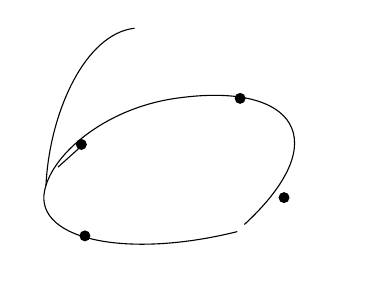
\begin{tikzpicture}[scale=.9]
\draw (0,0)..controls(-.25,-.75)and(1.1,-1.05)..(2.7,-.65);
\draw (2.8,-.55)..controls(4.1,.65)and(3.5,1.45)..(1.9,1.24)..controls(.9,1.12)and(.15,.5)..(0,0);
\fill (.5,.58) circle (2.2pt);\fill (2.74,1.23) circle (2.2pt);\fill (3.36,-.17) circle (2.2pt);\fill (.55,-.71) circle (2.2pt);
\draw (0,0)..controls(.05,1.03)and(.55,2.14)..(1.25,2.22);
\draw (.17,.26)--(.56,.61);
\end{tikzpicture}}

Le groupe des rotations du carré opère de façon simplement transitive sur l'ens $J$, de sorte que les $T_i$ s'identifient entre eux. Si $\omega_Q$ est l'ens des deux orientations du carré, \deleted{qui est \unsure{associé can.} $\unsure{1-1}$ \unsure{avec} l'ens $\omega_J$ des deux orientations de l'ens $J$,} on a un isom canonique
\[
T_i=\mathbb{U}\times_{\{\pm1\}}\omega_Q
\]
en choisissant comme origine \inserted{en $i$ associée à une orientation} la direction \uline{tangente}
\mspage{121}
